\documentclass[10pt,letterpaper]{article}
\usepackage[margin=0.78in]{geometry}
\usepackage{amsmath,amssymb,booktabs,array,enumitem,xcolor}
\usepackage[T1]{fontenc}
\usepackage{lmodern}
\usepackage{fancyhdr}
\usepackage{tikz}
\usetikzlibrary{arrows.meta}
\setlist[enumerate]{leftmargin=*,itemsep=0.7em,topsep=0.3em}
\pagestyle{fancy}
\fancyhf{}
\lhead{SYDE 556/750 \quad Handwritten Assignment 1}
\rhead{Worked solutions}
\cfoot{\thepage}
\setlength{\headheight}{14pt}
\newcommand{\R}{\mathbb{R}}
\newcommand{\vct}[1]{\boldsymbol{#1}}
\newcommand{\smallnote}[1]{{\color{black!65}\small #1}}
\begin{document}

\begin{center}
{\Large\bfseries Handwritten Assignment 1: Solutions}\\[3pt]
Neurons and Population Representation
\end{center}
\noindent These solutions use the normalized activity units stated in the assignment. Equivalent algebra and correctly labelled sketches receive the same conclusions; rounding may cause small differences.

\section*{1. Scalar ReLU neurons: encoding and tuning}
\begin{enumerate}[label=\textbf{1\alph*.}]
\item Subtracting the threshold equation from the maximum-current equation gives
\[
\boxed{\alpha=\frac{J_{\max}-J_{\mathrm{th}}}{1-\xi}},\qquad
\boxed{J^{\mathrm{bias}}=\frac{J_{\mathrm{th}}-\xi J_{\max}}{1-\xi}}.
\]
For ReLU, \(J_{\mathrm{th}}=0\) and \(J_{\max}=a^{\max}\), so \(\alpha=a^{\max}/(1-\xi)\) and \(J^{\mathrm{bias}}=-\alpha\xi\). Every \(J\leq0\) gives zero ReLU output, so \(G^{-1}(0)\) is not a single value. The boundary current is the intended value.

\item The gains are all \(100\), but the biases differ. In Hz:
\begin{center}\begin{tabular}{c r r r r r r r r r}\toprule
Neuron & \(\alpha\) & \(J^{\mathrm{bias}}\) & \(x=-1\) & \(-0.5\) & \(0\) & \(0.5\) & \(1\) & \(x=\xi/e\)\\\midrule
1 & 100 & 0 & 0 & 0 & 0 & 50 & 100 & 0\\
2 & 100 & 50 & 0 & 0 & 50 & 100 & 150 & \(-0.5\)\\
3 & 100 & 0 & 100 & 50 & 0 & 0 & 0 & 0\\
4 & 100 & 50 & 150 & 100 & 50 & 0 & 0 & \(0.5\)\\\bottomrule
\end{tabular}\end{center}
The course's named intercept \(\xi\) is in projected input \(u=e x\). On these \(x\)-axis plots the crossing is at \(x=\xi/e=e\xi\); for neuron 4, \(\xi=-0.5\) and \(e=-1\) give \(x=+0.5\).

\item A correct sketch joins the table values with straight active segments and horizontal zero segments. Neurons 1--2 rise rightward; 3--4 rise leftward. Each reaches its maximum at its preferred edge \(x=e\). With 16 sampled neurons, there are varied slopes, thresholds, and maxima, with roughly half rising in either direction.
\begin{center}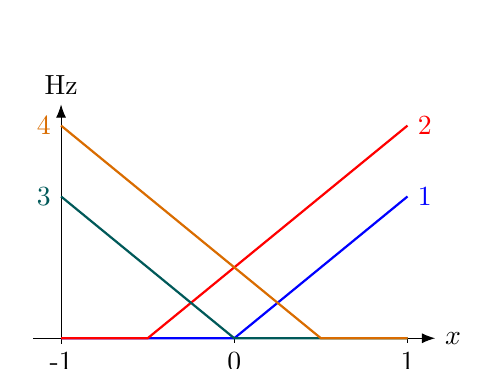
\begin{tikzpicture}[x=2.2cm,y=0.018cm,>=Latex]
  \draw[->] (-1.16,0) -- (1.16,0) node[right] {$x$};
  \draw[->] (-1,-4) -- (-1,165) node[above] {Hz};
  \foreach \x/\lab in {-1/-1,0/0,1/1} {\draw (\x,0) -- (\x,-3) node[below] {\lab};}
  \draw[blue,thick] (-1,0)--(0,0)--(1,100) node[right] {1};
  \draw[red,thick] (-1,0)--(-.5,0)--(1,150) node[right] {2};
  \draw[teal!70!black,thick] (-1,100) node[left] {3} --(0,0)--(1,0);
  \draw[orange!85!black,thick] (-1,150) node[left] {4} --(.5,0)--(1,0);
\end{tikzpicture}\end{center}
\end{enumerate}

\section*{2. Scalar identity decoding and noise}
\begin{enumerate}[label=\textbf{2\alph*.}]
\item Differentiating \(\|\vct{x}-\vct{d}^{T}A\|_2^2\) with respect to \(\vct{d}\) gives \((AA^T)\vct{d}=A\vct{x}\). Here
\[
AA^T=\begin{bmatrix}5&1\\1&5\end{bmatrix},\qquad
A\vct{x}=\begin{bmatrix}2\\-2\end{bmatrix},\qquad
\boxed{\vct{d}=\begin{bmatrix}1/2\\-1/2\end{bmatrix}}.
\]
The first neuron increases with \(x\), while the second decreases; their signed contributions must oppose each other to reconstruct \(x\).
\item \(\hat{\vct{x}}=(-1,0,1)\); signed errors are \((0,0,0)\) and RMSE is \(0\). The decoded plot lies on \(y=x\); the error plot is the zero line.
\item The supplied noisy test matrix gives \(\hat{\vct{x}}=(-1.25,0,1.25)\) and errors \((0.25,0,-0.25)\). The endpoints overshoot, and
\[
\mathrm{RMSE}=\sqrt{\frac{2(0.25)^2}{3}}=0.204.
\]
\item Differentiating the stated regularized objective gives
\[
\boxed{(AA^T+m\sigma^2 I)\vct{d}_{\mathrm{reg}}=A\vct{x}},\quad
m\sigma^2=3(0.5)^2=0.75,\quad
\vct{d}_{\mathrm{reg}}=\begin{bmatrix}8/19\\-8/19\end{bmatrix}.
\]
Clean testing gives \(\hat{\vct{x}}=(-16/19,0,16/19)\), errors \((-3/19,0,3/19)\), and RMSE \(\sqrt{2/3}(3/19)=0.129\). Noisy testing gives \(\hat{\vct{x}}=(-20/19,0,20/19)\), errors \((1/19,0,-1/19)\), and RMSE \(\sqrt{2/3}/19=0.0430\).
\begin{center}\begin{tabular}{lcc}\toprule Decoder & Clean-test RMSE & Noisy-test RMSE\\\midrule
Noise ignored & 0 & 0.204\\
Noise aware & 0.129 & 0.0430\\\bottomrule\end{tabular}\end{center}
The regularizer shrinks coefficients. This introduces some clean bias but reduces the effect of the particular noisy test realization. A different realization need not improve this much; the objective concerns expected noise error.
\end{enumerate}

\section*{3. Distortion and noise as population size grows}
\begin{enumerate}[label=\textbf{3\alph*.}]
\item Doubling \(n\) divides distortion by about \(4\), so its log-log slope is \(-2\): \(E_{\mathrm{dist}}\approx0.04(4/n)^2\). It divides noise error by \(2\), giving slope \(-1\): \(E_{\mathrm{noise}}=0.04(4/n)\). On separate log-log plots the distortion line is steeper.
\begin{center}\begin{tabular}{rccc}\toprule \(n\) & 128 & 256 & 512\\\midrule
\(E_{\mathrm{dist}}\) & \(3.91\times10^{-5}\) & \(9.77\times10^{-6}\) & \(2.44\times10^{-6}\)\\
\(E_{\mathrm{noise}}\) & \(1.25\times10^{-3}\) & \(6.25\times10^{-4}\) & \(3.13\times10^{-4}\)\\\bottomrule\end{tabular}\end{center}
\item With \(\vct{d}\) fixed, \(E_{\mathrm{noise}}=\sigma^2\sum_i d_i^2\) falls by \(10^2=100\). At \(n=16\) it becomes \(0.0100/100=0.000100\), which is 25 times smaller than \(E_{\mathrm{dist}}=0.00250\). Recomputing decoders changes their norm and usually reduces regularization, so both components can change; the simple factor of 100 applies only when decoders remain fixed.
\item Additional, differently tuned neurons provide a denser basis for approximating the identity; in this one-dimensional setting the illustrative distortion falls quadratically. Independent noise contributions average more slowly, giving the observed inverse-linear trend. Repeating with fresh populations reduces dependence on an unusually good or poor random draw.
\end{enumerate}

\section*{4. LIF rate neurons}
\begin{enumerate}[label=\textbf{4\alph*.}]
\item Above threshold,
\[
\frac{1}{a}=\tau_{\mathrm{ref}}-\tau_{\mathrm{RC}}\ln(1-1/J)
\quad\Longrightarrow\quad
\boxed{J(a)=\frac{1}{1-\exp[(\tau_{\mathrm{ref}}-1/a)/\tau_{\mathrm{RC}}]}}.
\]
Since \(J_{\mathrm{th}}=1\), the general gain/bias equations from 1a give
\(\alpha=(J(a^{\max})-1)/(1-\xi)\) and \(J^{\mathrm{bias}}=1-\alpha\xi\).
\item Here \((\tau_{\mathrm{ref}}-1/a^{\max})/\tau_{\mathrm{RC}}=-0.4\), so \(J_{\max}\approx3.033\), \(\alpha\approx2.033\), and \(J^{\mathrm{bias}}=1\). Therefore:
\begin{center}\begin{tabular}{r r rrrr}\toprule \(x\) & & \(-1\) & 0 & 0.5 & 1\\\midrule
\(J(x)\) && \(-1.033\) & 1 & 2.017 & 3.033\\
\(a(x)\), Hz && 0 & 0 & 63.7 & 100\\\bottomrule\end{tabular}\end{center}
The sketch is flat at zero through the threshold and then rises nonlinearly toward 100 Hz. With \(e=-1\), reflect it about \(x=0\). ReLU instead has a straight active segment; the LIF rate bends as current rises.
\item Here \(BB^T=I_2\) and \(B\vct{x}=(1,-1)^T\), so the unregularized decoder is \((1,-1)^T\). The regularization coefficient is \(m\sigma^2=3(0.2)^2=0.12\), giving
\(\vct{d}_{\mathrm{reg}}=(25/28,-25/28)^T\). Clean estimates are \((-25/28,0,25/28)\); noisy estimates are \((-15/14,0,15/14)\). The clean error plot has values \((-3/28,0,3/28)\); the noisy error plot has \((1/14,0,-1/14)\).
\begin{center}\begin{tabular}{lcc}\toprule Decoder & Clean-test RMSE & Noisy-test RMSE\\\midrule
Noise ignored & 0 & 0.163\\
Noise aware & 0.0875 & 0.0583\\\bottomrule\end{tabular}\end{center}
The corresponding \(\hat{x}\) sketches join the three estimate values against \(x=-1,0,1\) and include the ideal line \(\hat{x}=x\).
\end{enumerate}

\section*{5. A LIF neuron's two-dimensional tuning}
\begin{enumerate}[label=\textbf{5\alph*.}]
\item From 4b, \(J(\vct{x})=1+2.033\,\vct{e}\cdot\vct{x}\). Thus the rates at \(\vct{0},\vct{e},-\vct{e},\vct{e}_{\perp}\) are \(0,100,0,0\) Hz. The silent region is \(\vct{e}\cdot\vct{x}\leq0\), or \(x_1\leq x_2\); the threshold line is \(x_1=x_2\). Activity increases toward positive \(x_1\) and negative \(x_2\). The surface is flat over the silent half-disk and rises smoothly over the active half.
\begin{center}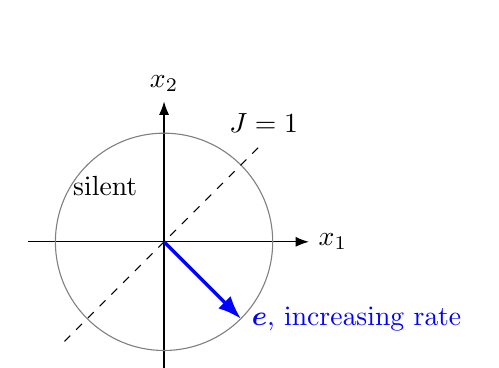
\begin{tikzpicture}[scale=1.15,>=Latex]
  \draw[->] (-1.5,0)--(1.6,0) node[right] {$x_1$};
  \draw[->] (0,-1.5)--(0,1.55) node[above] {$x_2$};
  \draw[gray] (0,0) circle (1.2);
  \draw[dashed] (-1.1,-1.1)--(1.1,1.1) node[above] {$J=1$};
  \draw[->,very thick,blue] (0,0)--(.85,-.85) node[right] {$\vct e$, increasing rate};
  \node at (-.65,.62) {silent};
\end{tikzpicture}\end{center}
\item The dot-product identity follows from \(\cos(A+B)=\cos A\cos B-\sin A\sin B\). Preferred angle is \(\theta=-\pi/4\pmod{2\pi}\), where rate is 100 Hz. The rate is zero where \(\cos(\theta+\pi/4)\leq0\), namely \(\theta\in[\pi/4,5\pi/4]\) in \([0,2\pi)\); it rises and falls on the complementary arc.
\item A plausible cosine fit uses \(c_2=1\) and \(c_3=\pi/4\) with positive amplitude. The underlying current has exactly this cosine dependence, but thresholding clips half the circle to zero and the LIF nonlinearity bends the active half. A single cosine cannot reproduce both features exactly.
\end{enumerate}

\section*{6. Vector populations and identity decoders}
\begin{enumerate}[label=\textbf{6\alph*.}]
\item Eight representative arrows have angles \(0,\pi/4,\ldots,7\pi/4\). For 100 neurons draw independent \(\phi_i\sim U[0,2\pi)\) and form \((\cos\phi_i,\sin\phi_i)\). Their arrows have unit length and roughly uniform directions with no systematic mean direction, although a finite random draw is not perfectly symmetric.
\item With neuron encoders in columns and training inputs in columns,
\[
E\in\R^{2\times100},\quad A\in\R^{100\times1600},\quad
X\in\R^{2\times1600},\quad D\in\R^{2\times100}.
\]
The matrix normal equation is \(D(AA^T+m\sigma^2I_{100})=XA^T\), hence
\[
\boxed{D=XA^T(AA^T+m\sigma^2 I_{100})^{-1}},\qquad \sigma=0.2\max(A).
\]
The clean tuning responses determine the mean signal and cross-neuron correlations. Independent zero-mean test noise is represented in the fitting objective by the regularizer, then separately sampled to assess performance.
\item For \(A=I_4\), \(X=E_4\), and \(m\sigma^2=4(0.2)^2=0.16\),
\(D=E_4/(1.16)=(25/29)E_4\). The four decoder arrows point along the same cardinal directions and each has length \(25/29\approx0.862\). General LIF activity is nonlinear and correlated, with unequal gains and intercepts; fitted decoding vectors may rotate and change length to correct those effects.
\end{enumerate}

\section*{7. Testing vector decoders and the population-vector rule}
\begin{enumerate}[label=\textbf{7\alph*.}]
\item Multiplying the supplied matrices gives
\[
\boxed{\hat X_D=\begin{bmatrix}0.96&0&-0.44\\0&0.48&-0.68\end{bmatrix}},\qquad
\boxed{\hat X_E=\begin{bmatrix}1&0.1&-0.6\\0.2&0.5&-0.8\end{bmatrix}}.
\]
The three target arrows end at \((1,0),(0,0.5),(-0.6,-0.8)\). On the same axes, mark the column endpoints above and draw arrows from the origin. Target magnitudes are \(1,0.5,1\). Encoder-decoded magnitudes are \(1.020,0.510,1\); fitted-decoder magnitudes are \(0.960,0.480,0.810\). The encoder rule preserves magnitude better in this particular example.
\item The raw squared-error sums are \(0.0500\) for \(E\) and \(0.0420\) for \(D\), over \(Nq=6\) coordinates. Thus
\[
\boxed{\mathrm{RMSE}_E=\sqrt{0.0500/6}=0.0913},\qquad
\boxed{\mathrm{RMSE}_D=\sqrt{0.0420/6}=0.0837}.
\]
For example, the first encoder estimate normalizes as
\((1,0.2)/\sqrt{1.04}=(0.981,0.196)\), while its target is \((1,0)\). The normalized columns are
\[
\hat X_E^{\mathrm{unit}}\approx\begin{bmatrix}0.981&0.196&-0.600\\0.196&0.981&-0.800\end{bmatrix},\qquad
\hat X_D^{\mathrm{unit}}\approx\begin{bmatrix}1&0&-0.543\\0&1&-0.840\end{bmatrix}.
\]
The normalized RMSEs are \(\boxed{0.114\text{ for }E}\) and \(\boxed{0.0282\text{ for }D}\). The fitted decoder preserves direction better here, even though its vector lengths are worse.
\item Testing varied radii exposes nonlinear rate changes and magnitude errors away from the training boundary; varied angles expose directional bias between preferred directions. In a broad, nearly uniform population, the encoder-weighted sum tends to point toward the stimulus because neurons tuned toward it fire more strongly and opposing directions roughly cancel. Encoders are simple and require no fitting. Fitted decoders account for actual tuning curves and correlations and usually yield lower reconstruction error, but require representative training data and a stable fit.
\end{enumerate}

\end{document}
